%% Dit is de domeinanalyse: Composite Objects %%
%% Freek 26 september: Een derde domeinanalyse zou kunnen gaan over hoe om te
%% gaan met Composite objects (bijv. hoe grafisch weer te geven, hoe op te
%% slaan in de data structuur)

\documentclass[a4paper,11pt,final]{article}

\usepackage[english]{babel}
\usepackage{graphicx}
\usepackage{hyperref}
\hypersetup{ colorlinks = true, citecolor = blue,linkcolor = blue }
\usepackage[a4paper]{geometry}
\usepackage{titlesec}% added to change section headers, see newcommand definition.
\usepackage{float}
\usepackage{wrapfig}


\bibliographystyle{alpha}

		

\begin{document}
\selectlanguage{english}
\begin{titlepage}
	\vspace*{\fill}
	\begin{center}
		\textsc{\large XMAS Model Designer (XMD)}\\[0.5cm]
		\textsc{\huge Qt Technologies}\\[0.5cm]
		\textsc{Stefan Versluys}\\ \textsc{\scriptsize 10/1/2015}\\[2.0cm]
	\end{center}
	\vspace*{\fill}
\end{titlepage}


\tableofcontents

\section{Introduction}
The XMAS Model Designer (xmd) is a graphical user interface (gui) used to design xmas models. 
Next to model design, it is also used to interact with the verification tools, persistence and 
some other functionality. 
This document describe the technical options offered by Qt and meet our
requirements.

\section{Declarative vs C++}
As in many deveopment environements today the trend is to put the gui in some kind 
of easy to read scripting while the logic or code behind is kept clean of gui styling.

\begin{wrapfigure}{r}{0.5\textwidth}
	\begin{center}
		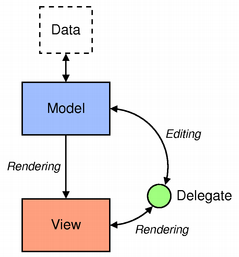
\includegraphics[width=0.30\textwidth]{modelview-overview.png}
	\end{center}
	\caption{Qt Quick Model View principle}
	\label{fig:modelview-overview}	
\end{wrapfigure}


Qt Modeling Language or QML is such a scripting or declarative language.
The advantage is that the logic , e.g. written in C++, purely represents
the data model. So no need to create separate gui classes in the code.
Of course, to make this possible such a data model must met some rules but these
are minor. E.g. to make a data model available for declarative use its
elements must inhire from specific objects. Properties, events or methods
that need to be exposed must be implemented via macros.
It has a low learning curve and in most cases just one line of
additional code. 

Qt Quick is the module that extends QML with C++. Figure~\ref{fig:modelview-overview}
shows a view-model of such a combination.
Using QML for gui makes the code smaller and much more maintainable.

The QML example below describes a fork primitive component. The keywords ``Component''
and ``Connector'' are in this case C++ classes of the data model behind. All kind of components
can be described in such a way even composites or even a whole model.
For a designer it is easy to describe a specific composite component and add an icon
to it. 
An other advantage of this setup is that it makes it possible to add a component editor 
in the future just because components are declarative and not hard coded.
\color{blue}
\begin{verbatim}
    {
	import QtQuick 1.1
	import XMAS 1.0
	
	Component {
	    id: comp
	    width: 200
	    height: 200
	    name: "fork"
	    connectors: [
	        Connector {
	            x: 5; y: 100
	            name: "a1"
	        },
	        Connector {
	            x: 195; y:40
	            name: "a2"
	
	        },
	        Connector {
	            x: 195; y:160
	            name: "a3"
	        }
	    ]
	    Image {source: "images/svgs/fork.svg"}
	}
    }
\end{verbatim}
\color{black}

This is just an example for the demo a full description of a component also needs the type property
(fork,merge,...), default label, context menu,...


A description of a whole model could be like

\color{blue}
\begin{verbatim}
{
    import QtQuick 1.1
    import XMAS 1.0
    
    Model {
        id: model
        version:1.5
        author:
        date:
        components:[
            Component{
                id:c1
                label: ``fork01''
                type: ``fork''
                x: 100; y:100 
                orientation: ``north''
            },
            Component{
                id:c2
                label: ``queue01''
                type: ``queue''
                x: 100; y:500 
                orientation: ``north''
                settings:[
                    Setting { key: ``size''; value: ''1''}
                ]
            },
        ]
        connections: [
            Connection {
                componentOut: ''c1''
                connectorOut: ``out1'' 
                componentIn: ''c2''
                connectorIn: ``in1''
            }
        ]
    }
}
\end{verbatim}
\color{black}

\section{Widget or not?}
Making canvas items as a widget makes it possible to add all kinds of user interface controls like checkbox 
or a lineedit. In Qt it is possible to do this via the QGraphicsProxyWidget but the question if this isn't overkill.
At this moment items are mostly a graphical image with a label and context menu. Those items are 
small and adding widgets will make these items bigger with is not a good idea. There will be also
an overhead for handling signals and making these properties persitent.
A canvas item is a graphical object with a label or lineedit and contextmenu to set the properties.

\section{Quick1 or Quick2?}
Whether to use Quick version 1 or 2 looks simple at first sight. But Quick 2 has a totally different approach
in building a graphical scene. It uses a dedicated scene graph based on OpenGL 2.0 instead of the
traditional imperative painting systems used in Quick 1 with the scene graph of the GraphicsView Framework.
The new quick 2 objects are incompatible with the graphicsview and cannot be used. 
On the other hand the new scene graph can not be used as a stand alone in c++ code and is pure
QML. 
Examine the quick 2 demo's , it seems that most examples are made in QML combined with javascript and 
C++ as code behind. Allthough there's an extra bit of javascript, it's amazing how a little piece of 
combined code languages can do such complex things.
The question is will it stay simple and little when using this new style for creating the XMAS Model Designer?
An other thing to keep in mind is the requirements of using c++ , so we keep 
QML to a minimum.
The Quick 2 graph scene is showed as something that can be used to design modern
user interfaces and as a replacement for quick 1 in the future. 

But if it comes to questions like how to put many 2D objects on a huge canvas as the graphicsview in 
Quick 1 can do, several forum answers tell to stay with the graphicsview framework.
The Quick 2 graph scene examples are all shown as a user interface that fits on a screen
with no scrolling area. Of course it must be possible but the risk is to high to bump into
limits or complexities while using it for the xmd tool.
In Qt 5.4 there's an example of a diagram editor , a user can put items on a scene
and connect those with an arrow. The example uses the graphicsview framework and not the 
new scene.
Quick 1 is still ok and the features xmd will use are basic drawing so no complex 3D transformation
or things like that. 


\section{Conclusion}
Quick 1 is not obsolete yet, it is not clear if Quick 2 can cover the functionality of the graphicsview.
Quick 1 can be simple ported to Quick 2 , instead of adding ``declarative'' tag in the Qt pro file
add ``quick'' and inhire from the QQML-objects instead of the QDeclarative-objects.

For now we will use Quick1 QML to separate GUI together with the graphicsview framework and
handle canvas objects as QDeclarativeItems which inhire from the QGraphicsItem.


\section{References}
\begin{itemize}
	\item \href{http://doc.qt.io/qt-5/qtquick-modelviewsdata-modelview.html}{Qt Model/View}
	\item \href{http://doc.qt.io/qt-5/qtquick-visualcanvas-scenegraph.html}{Qt Quick2 Scene Graph}
	\item \href{http://doc.qt.io/qt-5/graphicsview.html}{Graphics View Framework}
	\item \href{http://doc.qt.io/qt-5/qtquick-porting-qt5.html}{Porting Quick 1 to Quick 2}
	\item \href{http://blog.qt.digia.com/blog/2013/09/02/new-scene-graph-renderer/}{Graph performance}
\end{itemize}

\end{document}